\begin{center}
	\chapter{PROPOSED METHODOLOGY}
\end{center}
\justifying

\section{Preliminaries and Notation}

Let $\Sigma$ denote the alphabet of permutations from which input sequences are
drawn, and let $\langle \Sigma \rangle$ denote the group it generates under
composition. An input sequence is $g_1, g_2, \dots, g_T$ with $g_t \in \Sigma$,
and the target at position $t$ is the cumulative product
$g_1 g_2 \cdots g_t$.

A generalized Householder factor is
\begin{equation}
H(\beta, k) \;=\; I - \beta\, k k^{\!\top},
\qquad \lVert k \rVert = 1, \quad \beta \in [0, 2].
\end{equation}
It acts as the identity on the orthogonal complement of $k$ and scales the
component along $k$ by $(1 - \beta)$. Three values are distinguished:
$\beta = 0$ gives the identity, $\beta = 1$ the orthogonal projection that
removes the component along $k$, and $\beta = 2$ the reflection in the hyperplane
orthogonal to $k$.

The state-transition matrix applied at position $t$ is the product of $K$ such
factors, as in Equation \ref{eq:deltaproduct}. For a permutation $p$ of $n$
symbols, $\ell(p)$ denotes its transposition length, the least number of
transpositions whose product is $p$, and $c(p)$ the number of cycles in its cycle
decomposition, so that $\ell(p) = n - c(p)$.

Throughout, $K$ denotes the number of factors actually applied to a given token,
$n_h$ the maximum available, and $n_t$ the count that the adaptive layer assigns
to the token at position $t$.

\section{Reachability Bounds for Householder Products}

Two bounds constrain which transitions a product of $K$ factors can realise. Both
are established by explicit construction in double-precision arithmetic, with the
resulting matrices compared elementwise against their targets, so that neither
depends on the convergence of an optimiser.

\subsection{The rank bound}

Each factor differs from the identity by a matrix of rank one. A product of $K$
factors therefore satisfies
\begin{equation}
\operatorname{rank}(A - I) \;\le\; K .
\end{equation}
For a permutation matrix $P$ corresponding to the permutation $p$ of $n$ symbols,
\begin{equation}
\operatorname{rank}(P - I) \;=\; n - c(p) \;=\; \ell(p).
\end{equation}
Combining the two gives $K \ge \ell(p)$ as a necessary condition for exact
representation, and this holds for every admissible $\beta$, whether free or
fixed.

\subsection{The determinant-parity bound}

The determinant of a single factor is $\det H(\beta,k) = 1 - \beta$. When
$\beta$ is held at $2$, every factor is a reflection with determinant $-1$, so a
product of $K$ factors has $\det A = (-1)^K$, while a permutation matrix has
$\det P = (-1)^{\ell(p)}$. Exact representation therefore additionally requires
\begin{equation}
K \;\equiv\; \ell(p) \pmod 2 .
\end{equation}

The constructive reading of this bound is the one that matters for the design.
Realising a permutation of length $\ell$ using $K > \ell$ factors requires that
the surplus factors compose to the identity. With $\beta$ held at $2$ the only
available construction is a pair of identical reflections, which consumes two
surplus factors; with $\beta$ free, a single factor at $\beta = 0$ is already the
identity and consumes one. Consequently a free $\beta$ makes every $K \ge \ell$
reachable, whereas a fixed $\beta$ leaves half of all targets unreachable at any
given $K$.

This bound determines a design constraint stated in Section \ref{sec:mechanism}:
a mechanism that varies the effective factor count must scale a learnable
$\beta$ towards zero, and must not select between fixed values.

\section{The Order-Requirement Model}
\label{sec:demand}

The identification of the required factor count with the transposition length
$\ell$ rests on an assumption that is left implicit in the cost accounting of
prior work: that the matrix the layer must realise is the permutation matrix of
the symbol. This assumption is not necessary. The layer is required only to
maintain a state from which the cumulative product can be decoded, and it may
therefore realise $\rho(g)$ for any faithful representation $\rho$
\cite{serre} of the group generated by the alphabet. The choice of $\rho$
belongs to the layer.

Applying the rank bound under this freedom gives the requirement
\begin{equation}
D(g) \;=\; \min_{\rho \ \text{faithful on} \ \langle \Sigma \rangle}
\operatorname{rank}\bigl(\rho(g) - I\bigr).
\label{eq:demand}
\end{equation}

The consequences are most clearly seen on the alternating group $A_5$. Every
five-cycle is an even permutation, so an alphabet consisting only of five-cycles
generates $A_5$ rather than $S_5$. The group $A_5$ is isomorphic to the rotation
group of the icosahedron and therefore admits a three-dimensional faithful
representation, which $S_5$ does not. In $SO(3)$ every non-identity rotation
fixes exactly its axis, so $\operatorname{rank}(R - I) = 2$ for every
non-identity element, and by the Cartan--Dieudonn\'e theorem \cite{geometricalgebra} each such rotation
factors into exactly two reflections. A five-cycle therefore requires four
factors inside $S_5$ and two inside $A_5$.

Table \ref{table:demand} records the requirement for the groups relevant to this
work, together with the range of transposition lengths, showing where the two
quantities diverge.

\begin{table}[ht]
	\caption{Order requirement by generated group}
	\centering
	\begin{tabular}{c c c c c}
		\hline\hline
		Group & $|G|$ & Min.\ faithful dim. & $D$ over non-identity & $\ell$ range \\ [0.5ex]
		\hline
		$S_3$ & 6 & 2 & 1, 2 & 1--2 \\
		$S_4$ & 24 & 3 & 1, 2, 3 & 1--3 \\
		$A_4$ & 12 & 3 & 2 only & 2 \\
		$A_5$ & 60 & 3 & 2 only & 2--4 \\
		$S_5$ & 120 & 4 & 1, 2, 3, 4 & 1--4 \\ [1ex]
		\hline
	\end{tabular}
	\label{table:demand}
\end{table}

Two consequences follow, and both are used in the experimental design.

The first is that the requirement is a property of the alphabet, not of the
symbol. Augmenting an alphabet of five-cycles with a single transposition closes
it over $S_5$ instead of $A_5$. The three-dimensional faithful representation is
no longer available, the minimum faithful dimension rises to four, and the
requirement of every five-cycle in the alphabet rises from two to four. The
cheapest symbol available raises the cost of every other symbol. No model of
per-symbol difficulty can reproduce this behaviour, and it provides a sharp
prediction that Section \ref{sec:design} operationalises as an experiment.

The second is that the proposed mechanism has a well-defined region of
applicability, identifiable before any model is trained. Where $D$ is constant
across the non-identity elements of the alphabet, as it is for $A_4$ and $A_5$,
per-token allocation cannot reduce computation at all, because every symbol
requires the same order. Adaptive allocation is beneficial exactly when the
distribution of $D$ over the alphabet is dispersed.

\section{Adaptive-Order Architecture}
\label{sec:mechanism}

\subsection{The halting gate}

A small feed-forward network reads the layer input at each position and emits
$K$ halting values $\lambda_t^{1}, \dots, \lambda_t^{K}$ in $(0,1)$. The gates
applied to the individual factors are their cumulative products,
\begin{equation}
g_t^{i} \;=\; \prod_{j \le i} \lambda_t^{j},
\qquad\text{so that}\qquad
g_t^{1} \ge g_t^{2} \ge \dots \ge g_t^{K},
\end{equation}
which makes the gate monotone: once a factor is disabled, no later factor is
re-enabled, and the allocation is therefore described by the single quantity
\begin{equation}
n_t \;=\; \sum_{i=1}^{K} g_t^{i}.
\end{equation}

The gate is applied to the factor strength rather than to the factor itself,
\begin{equation}
\tilde{\beta}_t^{\,i} \;=\; g_t^{i} \cdot \beta_t^{i},
\end{equation}
with the multiplication performed after the $2\,\sigma(\cdot)$ nonlinearity that
produces $\beta$. A gate value of zero therefore drives $\beta$ to zero, and the
corresponding factor becomes exactly the identity. This placement is required by
the determinant-parity bound: a mechanism that instead selected between fixed
values of $\beta$ would leave the parity constraint in force and render half of
all targets unreachable at any given factor count.

The gate is evaluated in a soft mode during training, where the cumulative
products are used directly and gradients are smooth, and in a hard mode at
evaluation, where the gates are thresholded to $\{0,1\}$ with a straight-through
estimator. All reported allocations are obtained in hard mode, so that a reported
cost is an integer count of factors rather than a sum of sigmoids.

Figure \ref{fig:mechanism} shows the arrangement.

\begin{figure}[ht]
	\centering
	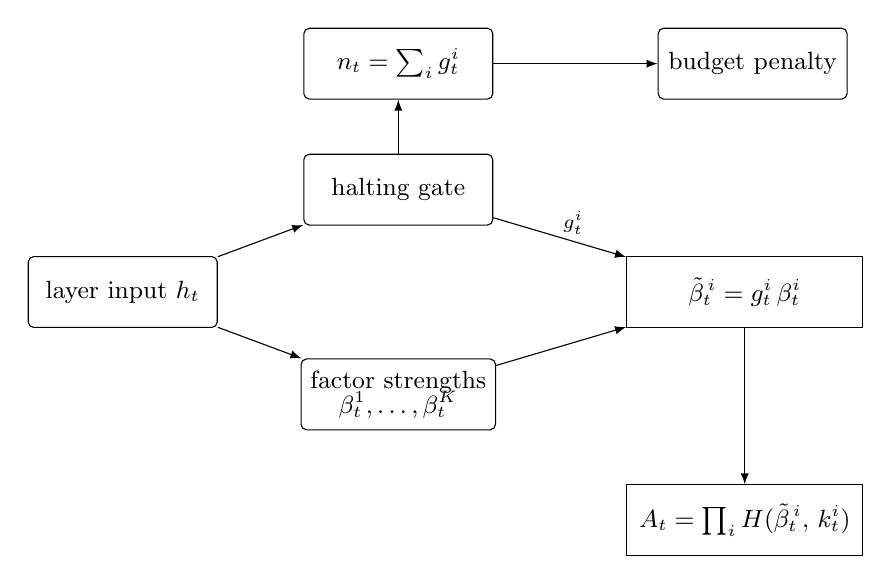
\begin{tikzpicture}[
		box/.style = {draw, rounded corners=2pt, minimum width=24mm, minimum height=9mm, align=center, font=\small},
		fac/.style = {draw, minimum width=30mm, minimum height=9mm, align=center, font=\small},
		>=latex
	]
	\node[box] (nt)   at (3.5,2.9)  {$n_t=\sum_i g_t^{i}$};
	\node[box] (bud)  at (8.0,2.9)  {budget penalty};
	\node[box] (gate) at (3.5,1.3)  {halting gate};
	\node[box] (h)    at (0,0)      {layer input $h_t$};
	\node[box] (beta) at (3.5,-1.3) {factor strengths\\[-2pt]$\beta_t^{1},\dots,\beta_t^{K}$};
	\node[fac] (mul)  at (7.9,0)    {$\tilde{\beta}_t^{\,i} = g_t^{i}\,\beta_t^{i}$};
	\node[fac] (prod) at (7.9,-2.9) {$A_t=\prod_i H(\tilde{\beta}_t^{\,i},\,k_t^{i})$};

	\draw[->] (h) -- (gate);
	\draw[->] (h) -- (beta);
	\draw[->] (gate) -- node[above right, font=\scriptsize, inner sep=1pt] {$g_t^{i}$} (mul);
	\draw[->] (beta) -- (mul);
	\draw[->] (mul) -- (prod);
	\draw[->] (gate) -- (nt);
	\draw[->] (nt) -- (bud);
	\end{tikzpicture}
	\caption{The adaptive-order layer. The halting gate emits monotone gates that scale the factor strengths; the sum of the gates is the token's effective order and is the quantity the budget penalty acts upon.}
	\label{fig:mechanism}
\end{figure}

\subsection{Training objective}

The layer is trained on the sum of the task loss and a penalty on the mean
effective order,
\begin{equation}
\mathcal{L} \;=\; \mathcal{L}_{\text{task}} \;+\; \gamma(s)\,\overline{n},
\qquad
\overline{n} \;=\; \frac{1}{BT}\sum_{b,t} n_{b,t},
\end{equation}
where $\gamma(s)$ is the budget weight at training step $s$. No term in this
objective references the correct allocation; the gate receives no supervision on
$n_t$ and must infer it from the interaction between the two terms, the task loss
opposing closure where expressivity is needed and the penalty favouring closure
everywhere else.

The gate is initialised open, so that at the first step the layer is exactly a
fixed-order model with $K = n_h$, which is the configuration known to converge.
The budget weight is held at zero for a warm-up period and then increased
linearly to its final value, so that the gate cannot close before the task has
been learned:
\begin{equation}
\gamma(s) \;=\;
\begin{cases}
0, & s \le s_{\text{warm}},\\[2pt]
\gamma \cdot \min\!\left(1, \dfrac{s - s_{\text{warm}}}{s_{\text{ramp}}}\right), & s > s_{\text{warm}} .
\end{cases}
\end{equation}
A configuration with $\gamma = 0$, in which the gate is present and trained but
never penalised, serves as the control for the effect of the gate's presence
alone.

\section{Cost Accounting and Execution Strategy}

The implementation evaluated here expands all $n_h$ factors and multiplies the
disabled ones by zero. This is numerically exact, and it is the strategy under
which every cost figure in this work is obtained. Accordingly, cost is reported
throughout as \emph{required work per token}, defined as the mean number of
factors whose gate is open at evaluation,
\begin{equation}
\text{cost} \;=\; \frac{1}{|\mathcal{T}|}\sum_{t \in \mathcal{T}} n_t ,
\end{equation}
where $\mathcal{T}$ ranges over positions carrying a group element, special
tokens being excluded because their correct transition is the identity. Under the
dense strategy a reduction in this quantity does not by itself reduce elapsed
time; converting it into elapsed time requires a ragged execution strategy in
which disabled factors are not materialised, and that is a subject of continuing
work.

\section{Experimental Design}
\label{sec:design}

\subsection{Data}

Sequences of length $k = 128$ are generated over a chosen alphabet of
permutations of five symbols, with the target at each position the cumulative
product of all symbols up to and including that position. Unless stated
otherwise, $100{,}000$ sequences are used for training and $2{,}000$ held out for
evaluation.

Two families of alphabet are used. The first is a mixture family, containing ten
transpositions and twenty-four five-cycles, in which a mixture parameter $p$
controls the fraction of five-cycles; the generated group is $S_5$ for every
$p < 1$, so the requirement is four for a five-cycle and one for a transposition,
and the expected requirement is $E[D] = 1 + 3p$. The second is a closure family,
in which the alphabet is varied so that the generated group changes while the
symbols themselves are held as similar as possible; this family operationalises
the prediction of Section \ref{sec:demand}, since alphabets of comparable size
fall on either side of the $A_5$/$S_5$ boundary.

\subsection{Model and optimisation}

All experiments use a single layer with twelve heads of dimension thirty-two and
hidden width $128$, in bfloat16. Optimisation is by AdamW at a constant learning
rate of $10^{-3}$, batch size $128$, for $20{,}000$ steps unless stated
otherwise. Experiments are run on an NVIDIA RTX 4050 Laptop GPU with 6\,GB of
memory.

\subsection{Arms and controls}

Three conditions are compared, and where they appear together they are trained
within a single invocation so that no comparison depends on a figure recorded
elsewhere.

\begin{enumerate}[label={(\arabic*)}]
	\item \textbf{Fixed order.} The unmodified layer at a constant $n_h$. Cost is
	$n_h$ by construction.
	\item \textbf{Oracle allocation.} The adaptive layer with gates supplied from
	ground truth, so that $n_t = D(g_t)$ exactly. This condition uses the same
	architecture and the same parameter count as the fixed-order arm at
	$n_h = 4$, differing only in the computation spent, and it establishes the
	best allocation attainable rather than the allocation a learned gate produces.
	\item \textbf{Learned allocation.} The adaptive layer with the halting gate
	trained under the budget penalty and no supervision on $n_t$.
\end{enumerate}

\subsection{Metrics}

Token accuracy is the fraction of positions predicted correctly. Sequence
accuracy requires every position of a sequence to be correct and is
correspondingly stricter: at $k = 128$, per-position accuracy of $0.99$
corresponds to sequence accuracy of $0.28$.

For the adaptive conditions, the allocation is evaluated against the requirement
$D$ of Equation \ref{eq:demand}, clipped to the factor count available. Three
quantities are reported. The mean absolute allocation error is
$\frac{1}{|\mathcal{T}|}\sum_t |n_t - D(g_t)|$. The under-allocated and
over-allocated fractions are reported separately rather than combined, since
under-allocation removes expressivity the task requires whereas over-allocation
only expends computation. Finally, the mean of $n_t$ is reported \emph{grouped by
the requirement} $D$, which distinguishes a gate that tracks the requirement from
one that reaches the same average by closing uniformly across all tokens.

\subsection{Measurement protocol}

The bfloat16 kernels used by the implementation employ non-deterministic atomic
accumulation, so repeated runs of an identical configuration are not bitwise
identical. On configurations that solve reliably this produces a spread of
approximately $0.005$ in token accuracy and $0.05$ in sequence accuracy. On the
configurations characterised in Section 4.6 the outcome distribution is bimodal
and the spread is far larger, with identical configurations producing token
accuracies of $0.1177$ and $0.9598$. On such configurations the summary statistic
reported is the fraction of runs that escape the loss plateau, taken over
repeated runs, rather than a mean.

Every experiment is accompanied by a self-test that evaluates its measurement
code against synthetic inputs whose correct output is known in advance, and each
such test is confirmed to fail when run against a deliberately incorrect
implementation.
\null
